\documentclass[letterpaper]{article}

% authors and affiliations
\title{PMoveSTIR---A general framework to incorporate movement and space use information in epidemiological models}
\usepackage{authblk}
\author{Juan S. Vargas Soto \and Mark Q. Wilber}
\affil{School of Natural Resources, University of Tennessee, Knoxville, TN}
\date{}


\usepackage[english]{babel}
\usepackage[utf8x]{inputenc}
\usepackage{amsmath}
\usepackage{graphicx}
\usepackage[left=1 in, right=1 in, top=1 in, bottom=1 in]{geometry}
% \usepackage{hyperref}
\usepackage{bbold}
\usepackage{rotating}
\usepackage{bbm}
\usepackage{array}
\newcolumntype{C}[1]{>{\centering\arraybackslash}m{#1}}
% \usepackage{kbordermatrix}
\usepackage{footnote}
\makesavenoteenv{tabular}
\makesavenoteenv{table}
% \renewcommand{\theequation}{{S}\arabic{equation}}

\makeatletter
% \addto\captionsenglish{%
%   \renewcommand{\fnum@figure}{Figure S\thefigure}%
%   \renewcommand{\fnum@table}{Table S\thetable}%
% }
\makeatother

% Bibliography
\usepackage[round, colon]{natbib} % Bibliography - APA
\bibliographystyle{abbrvnat}
%\bibpunct{(}{)}{;}{a}{}{,}

% Line numbers
\usepackage{lineno}
%\def\linenumberfont{\normalfont\footnotesize\ttfamily}
%\setlength\linenumbersep{0.2 in}

\usepackage{setspace}

\newcommand{\ignore}[1]{}

\begin{document}


\maketitle

\linenumbers
\doublespacing

\section*{Introduction}

Individual movement is among the most critical factors that determine the possibility of transmission of parasites and infectious disease \citep{Manlove2022,Dougherty2022}. At the landscape scale, the combination of individual movements defines how parasites and infectious disease spread through the landscape \citep{Fofana2017}. At a more local scale, how an animal moves determines whether they come into contact with other individuals of the same and other species, or with parasites in the environment, as well as where these contacts occur, and how often. These contacts are the component of transmission that is most influenced by environmental drivers (the other component being probability of transmission given contact). Yet movement itself is the product of a complex interaction between resource availability, physiology, landscape features, inter- and intraspecific interactions \citep{Nathan2008,Merkle2018,Vanderwaal2017}, and it can be hard to disentangle their influence. Understanding mechanistically how movement influences transmission risk, and formally linking environmental drivers of movement with transmission risk, remain outstanding tasks in disease ecology \citep{White2018}. 

To understand how movement impacts epidemiological dynamics, we first need to properly characterize movement. Substantial technological advances now make it possible to track a wide diversity of animal species with high spatial and temporal resolution. At the same time, the development of analytic methods for these increasingly detailed data make it possible to infer/interpolate missing locations based on biological processes, to define the utilization distribution across the landscape, and to link movement with behavior and environmental factors \citep{Signer2017,Hooten2017,Avgar2015}. Similarly, we can use fine-scale spatiotemporal data to infer where and when contact between animals occurs \citep{Noonan2021}, and to build contact networks for direct \citep{Craft2015} and indirect interactions \citep{Yang2023}. These indirect interactions are particularly important in the context of disease transmission, given that many parasites can persist in the environment, which can lead to transmission without direct contact between hosts. Integrating these indirect interactions can drastically reshape disease transmission networks and the inferences about epidemiological dynamics \citep{Wilber2022,Richardson2015}. 

% Rough additions and thoughts from Mark highlighting key knowledge gaps

The utilization distribution (UD) plays a central role in linking host movement to contact, and transmission.  The UD describes the probability that a host uses a particular area on a landscape and can reflect the long-run or a transient distribution of habitat use (Tao). Methods have been developed to predict utilization distributions directly from spatial and social factors driving movements and continuous-time movement models can be used to calculate biologically realistic utilization distributions [Potts citation, Flemming citation].  There wide-spread use and biological underpinnings mean that UDs are an essential tool for linking animal movement and transmission.  Moreover, because UDs can be directly linked to environmental drivers of movement [citations], they have the potential to predict contact and transmission in novel environments and can also be used for prospective analyses to understand how the effects of environmental and social perturbations cascade across scales, from individual movement to population and landscape-level disease transmission.  This has important implications for understanding the spread and persistence of wildlife disease and predicting spillover risk.  However, while studies have often used metrics such as home range overlap to build contact networks, only recently have studies formally linked UDs with animal contacts. 

One such approach developed by Noonan et al. showed how UDs could be used to predict the conditional distribution of encounters (CDE) between pairs of individuals. CDE does X, Y and Z. While the work by Noonan et al is a key advance in linking empirical movement to contact, two key challenges remain when linking UDs to disease transmission.  First, while the CDE provides a spatial distribution of encounter probability based on the overlap of utilization distributions, the resulting output of the CDE (a probability density function with units per $area$) does not describe an epidemiological contact - a contact with components of contact formation, contact duration, pathogen acquisition, pathogen shedding, and pathogen decay.  [Mention that an epidemiological contact would ideally be described in terms of force of infection with units per time or per area per time, not something the CDE does].  Moreover, the CDE does does not explicitly consider both direct and indirect contacts, which can be highly relevant for disease spread in a population. The second challenge is that the CDE ignores correlation in host movement [rephrase].  While a useful simplification (and one that we will also use throughout this study), it is unclear how much this assumption might change how individual UDs can be used to predict epidemiological contact.  

The MoveSTIR framework, developed by \citet{Wilber2022}, provides a generalizable model for leveraging spatially and temporally explicit movement data to understand epidemiological dynamics. This framework is defined explicitly in terms of epidemiological processes, allowing to tease apart individual contributions to the overall transmission across the population, to other specific individuals, or to specific locations. The theoretical framework should also be flexible enough to use different types of data like GPS collars, proximity loggers, or camera-traps \citep{Wilber2022}. 
Calculating the full transmission kernel can be computationally costly, and this cost increases with finer temporal resolution—observed or interpolated, with more individuals, and with longer tracking time. Depending on the study system, a more general approach with simplifying assumptions could capture the epidemiological dynamics in a similar way. 

% Previous research has tried to infer contact from the spatial overlap between individuals. E.g. KDE overlap as a measure of FOI (XXX, XXX).
% Different movement histories could lead to different transmission dynamics if movement of individuals is somehow correlated (e.g. due to avoidance/attraction). Incorporating the temporal history of locations can also reveal asymmetric potential of acquiring parasites. These factors have been explored in the moveSTIR paper \citep{Wilber2022}. This framework reveals the importance of accounting for indirect transmission.

% <!--# This language is very vague right now, need to fix and clarify -->

Here, we generalize the moveSTIR model for multiple scenarios. Our goal is to develop a common framework that captures a majority of study cases related to wildlife movement and disease transmission, and that can make use of different data streams (e.g. GPS tracking, proximity/contact loggers, camera-traps). 
%Putting the moveSTIR transmission kernel in a similar framework to existing methods of movement analysis (e.g. SSF) could facilitate linking mechanistically environmental variables with the transmission process. 
We develop the general analytic framework and the different special cases, explore benefits and implications of particular cases using simulations, and apply our framework to observed data for representative study systems.

\section*{Methods}

\subsection*{Linking utilization distributions to transmission through PMoveSTIR}

Consider two individuals, $i$ and $j$, moving and interacting across a landscape.  We want to ask: on average across space and time what is the potential or realized force of infection (FOI) host $i$ feels from host $j$ in some location $x$?  The FOI is an essential quantity to estimate in disease ecology that underlies our ability to predict the spread of disease across populations and landscapes. Here we develop the approach PMoveSTIR that formally links host utilization distributions, direct and indirect contacts, and spatial estimates of force of infection.

PMoveSTIR builds on the recently developed MoveSTIR model. In MoveSTIR and PMoveSTIR we assume that transmission happens by one host depositing pathogen into the environment and another host picking that pathogen up.  Deposition and acquisition can represent a range of processes, from one individual coughing and another inhaling in a matter of seconds to one host depositing parasite eggs in the environment and another individual consuming these eggs days or weeks later. This fairly general assumption encompasses standard density-dependent transmission as a special case \citep{Cortez2021}. Moreover, considering transmission through deposition and acquisition components clearly links direct transmission and indirect transmission along a continuum \citep{Wilber2022}.

Given these transmission assumptions, we can define the pairwise force of infection felt by host $i$ in location $x$ from host $j$ at time $t$ as \citep{Wilber2022}

\begin{equation}
    h_{i \leftarrow j}(t, x) = \int_{-\infty}^{t} \beta' \lambda \delta_{x_j(u)}(x) \delta_{I_j(u)}(I) S(t - u) du
    \label{eq:original_foi}
\end{equation}
where $\beta'$ is the pathogen acquisition rate of host $i$, $\lambda$ is the pathogen deposition rate of host $j$, $\delta_{x_j(u)}(x)$ is an indicator variable that is one if host $j$ is in location $x$ at time $u$ and zero otherwise, $\delta_{I_j(u)}(I)$ is an indicator function that is one if host $j$ is in an infected state at time $u$ and zero otherwise, and $S(t - u)$ is probability that any pathogen deposited at time $u < t$ is still alive at time $t$ \citep[see][for a full derivation]{Wilber2022}.  Moving forward we will make an assumption of maximum transmission risk and assume that host $j$ is always infected. This is equivalent to building a contact network and also represents the structural form of FOI needed to compute pathogen invasion thresholds \citep{Wilber2022}.  Note that equation \ref{eq:original_foi} encompasses both direct contact when $u \approx t$ and indirect contact when $u < t$.

It is beneficial to consider the interpretation of ``contact'' and the parameter $\beta'$.  First, we assume that contact can occur when both individuals are in location $x$ with area $A_x$.  We could also think about location $x$ being a habitat patch or a grid cell, such that contact can only occur when two hosts are within the habitat patch or grid cell. Importantly, we assume that locations $x$ on the landscape do not overlap such that summing locations $x$ equals some total area over which individuals can move. Alternatively, we could define a contact as occurring whenever two hosts are within some distance $r$ \citep{Wilber2022}.  Under both of these interpretations, a key assumption is that the likelihood of contact is uniform within the area $A_x$, consistent with a so-called top hat encounter function \citep{Gurarie2013,Wilber2022}.

The term $\beta'$ is the rate at which host $i$ picks up pathogen within the location $x$ and can be re-written as $\tilde{\beta} / A_x$, where $\tilde{\beta}$ has units area units / time (e.g., $m^2 / \text{day}$) and $A_x$ gives the area of location $x$ (e.g., 10 $m^2$). Therefore, the total acquisition rate scales with the area in which contact can occur. In a large area, the same amount of pathogen deposited by host $j$ would be spread over a larger area (or, equivalently, host $i$ would have to traverse a larger area to find the ``packet'' of pathogen), reducing total acquisition rate of host $i$ and the corresponding force of infection.  When using PMoveSTIR, it is critical to be specific about our definition of contact and the area units associated with $\beta'$.  

Returning to \ref{eq:original_foi}, this equation forms the backbone of the previously describe MoveSTIR \citep{Wilber2022} and assumes we know  the trajectory of host $i$ and host $j$. Given the increasing wide availability of fine-scale movement data and tools in movement ecology, this is often approximately true over some finite time interval. However, as we move toward predicting contacts and transmission beyond the time intervals and locations over which we observe animal movement, it is more useful to consider a probabilistic version of equation \ref{eq:original_foi}, where we only know, with some probability, where host $i$ and $j$ are at any point in time.  In the language of Alston et al. 2022 (BioRXiv), PMoveSTIR works with the range distribution of an animal while MoveSTIR works with the occurrence distribution.  

Considering probabilistic movements, we can re-write equation \ref{eq:original_foi} as

\begin{equation}
    h_{i \leftarrow j}(t, x) = \int_{-\infty}^{t} \beta' \lambda \delta'_{x_i(t)}(x) \delta'_{x_j(u)}(x) S(t - u) du
    \label{eq:prob_foi}
\end{equation}
where $\delta'_{x_i(\tau)}(x)$ and $\delta'_{x_j(\tau)}(x)$ are random variables that specify whether or not (i.e., 0 or 1) host $i$ or host $j$ is in location $x$ at time $\tau$ (e.g., in a grid cell).  This means that $h_{i \leftarrow j}(t, x)$ is also a random variable. Taking the expectation of $h_{i \leftarrow j}(t, x)$ with respect to repeated, hypothetical simulations of animal movement we obtain

\begin{equation}
    E[h_{i \leftarrow j}(t, x)] := h^*_{i \leftarrow j}(t, x) = \int_{-\infty}^{t} \beta' \lambda E[\delta'_{x_i(t)}(x) \delta'_{x_j(u)}(x)] S(t - u) du.
    \label{eq:expected_foi}
\end{equation}

Interpreting this expectation, we are asking: if we simulated some movement process thousands of times, what is the probability that host $i$ is in location $x$ at time $t$ and host $j$ was in location $x$ at a previous time $u$? 

\subsection*{Linking equation \ref{eq:expected_foi} to utilization distributions}

Our goal is to understand how utilization distributions link to spatio-temporal transmission risk.  To do that, first note that if $Y$ and $Z$ are two random variables, then $E[YZ] = E[Y]E[Z] + Cov(Y, Z)$.  We can therefore write equation \ref{eq:expected_foi} as

\begin{equation}
    \begin{aligned}
        h^*_{i \leftarrow j}(t, x) &= \int_{-\infty}^{t} \frac{\tilde{\beta}}{A_x} \lambda E[\delta'_{x_i(t)}(x) \delta'_{x_j(u)}(x)] S(t - u) du \\
        &= \frac{\tilde{\beta}}{A_x} \lambda \int_{-\infty}^{t} [E[\delta'_{x_i(t)}(x)] E[\delta'_{x_j(u)}(x)] + Cov(\delta'_{x_i(t)}(x), \delta'_{x_j(u)}(x))] S(t - u) du \\
        &= \frac{\tilde{\beta}}{A_x} \lambda \int_{-\infty}^{t} [p_i(x, t) p_j(x, u) + Cov(\delta'_{x_i(t)}(x), \delta'_{x_j(u)}(x))] S(t - u) du \\
    \end{aligned}
    \label{eq:foi_cov}
\end{equation}
where we use the fact that the expectation of an indicator variable is a probability \citep{Grimmett2001}. The terms $p_i(x, t)$ and $p_j(x, t)$ give the probabilities that host $i$ and $j$ are in location $x$ as time $t$ and can also be written as $p_i(x, t) = \int_{A_x} f_i(s, t) ds$ where $f_i(s, t)$ is the probability density of host $i$ using the point $s$ at time $t$ and integral is over the area $A_x$ (defined equivalently for host $j$). Thus, $f_i(s, t)$ and $f_j(s, u)$ are the transient utilization distributions of host $i$ and host $j$ and equation \ref{eq:foi_cov} shows how they relate to spatio-temporal FOI.

% Second, we could write equation \ref{eq:expected_foi} as 

% \begin{equation}
%     \begin{aligned}
%     h^*_{i \leftarrow j}(t, x) &= \int_{-\infty}^{t} \beta' \lambda E[\delta'_{x_i(t)}(x) \delta'_{x_j(u)}(x)] e^{-\nu(t - u)} du \\
%     &= \beta' \lambda \int_{-\infty}^{t} p(i \in x \text{ at } t, j \in x \text{ at } u) e^{-\nu(t - u)} du) \\
%     &= \beta' \lambda \int_{-\infty}^{t} p(i \in x \text{ at } t | j \in x \text{ at } u) p(j \in x \text{ at } u) e^{-\nu(t - u)} du \\
%     \end{aligned}
%     \label{eq:foi_prob}
% \end{equation}

To better understand the meaning of equation \ref{eq:foi_cov}, consider the special case of statistical stationarity in movement (i.e., the mean location are constant through time, though animal is still moving).  For clarity, also assume that pathogen survival in the environment follows $S(t - u) = e^{-\nu (t - u)}$, where $\nu$ is the pathogen decay rate.  We  can simplify equation \ref{eq:foi_cov} to (derivation in SI)

\begin{equation}
    \begin{aligned}
    E[h_{i \leftarrow j}(x)] = \frac{\tilde{\beta}}{A_x} \lambda [p_i(x)p_j(x) \frac{1}{\nu} + \int_{0}^{\infty} Cov(\delta_{i \in x}, \delta_{j \in x} | \tau) e^{-\nu \tau} d\tau]
    \end{aligned}
    \label{eq:foi_stationary}
\end{equation}
The key insight here is that, given a stationary assumption, the expected force of infection in location $x$ depends on i) the marginal probabilities that host $i$ and host $j$ use location $x$, where $p_i(x) = \int_{A_x} f_i(s) ds$ and $p_j(x) = \int_{A_x} f_j(s) d$ and $f_i$ and $f_j$ are the utilization distributions of host $i$ and $j$ and ii) the covariance in how host $i$ and host $j$ use location $x$ at different time lags $\tau$. For example, if host $i$ and $j$ always use location $x$ together (a positive correlation at time lag $\tau = 0$), this will increase the force of infection relative to the product of their utilization distributions.  

To gain some intuition into equation \ref{eq:foi_stationary}, consider the case of two hosts moving independently across a landscape.  Because hosts are moving independently, the covariance is zero such that $\frac{\tilde{\beta}}{A_x} \frac{\lambda}{\nu} p_i(x)p_j(x)$ -- the expected FOI experienced by two hosts is exactly proportional to the products of their utilization distributions \citep[similar to the result given in][]{Noonan2021}.  In this particular case the FOI is symmetrical, i.e. the FOI from $i$ to $j$ is the same as from $j$ to $i$.

Now assume hosts are moving independently and use space uniformly on a gridded landscape and contact occurs when individuals are in the same grid cell.  The area of grid cell $x$ is $A_x$ and the total area of the landscape is $A_{tot} = n A_x$, where $n$ is the number of grid cells that comprise $A_{tot}$. Because movement is random with respect to location, $p_i(x) = p_j(x) = \frac{A_x}{A_{tot}}$ and the force of infection at location $x$ is $\frac{\tilde{\beta}}{A_{tot}} \frac{\lambda}{\nu} \frac{A_x}{A_{tot}}$.  Finally, if we want the expected FOI from $j$ to $i$ over all space, we sum over all grid cells and get $\frac{\tilde{\beta}}{A_{tot}} \frac{\lambda}{\nu}$. This is exactly equivalent to the FOI we would expect using a mass action assumption of hosts moving independently and transmitting within an area $A_{tot}$ \citep{McCallum2001}.

% Instead of assuming hosts are moving uniformly across all $n$ grid cells, assume that they only occupy one grid cell on the landscape.  Now $p_i(x) = p_j(x) = 1$ if $x$ is the grid cell they use and is zero otherwise.  Applying the same steps and summing over all space we get $\frac{\tilde{\beta}}{A_{x}} \frac{\lambda}{\nu}$ -- the FOI from $j$ to $i$ is what we would expect if hosts were moving uniformly over a smaller area $A_x$. 

\subsection*{Applying equation \ref{eq:foi_cov} under different degrees of spatial and temporal heterogeneity}

Equation \ref{eq:foi_cov} is the most general formulation of PMoveSTIR. However, as we did in our example of statistically stationary movement above, it is useful to consider different degrees of spatial and temporal heterogeneity and how they simplify/modify equation \ref{eq:foi_cov}. This allows us to link different metrics such as temporally varying utilization distributions, stationary utilization distributions, and home range overlap to force of infection. In Fig. 1, we show how PMoveSTIR provides a general approach for accounting for different degrees of spatial and temporal heterogeneity in movement.

\subsubsection*{The upper right-hand corner: Heterogeneous space and time}

The upper right-hand corner is the most general case captured by equation \ref{eq:foi_cov} -- utilization distributions and between-individual spatial covariance are time-varying and heterogeneous in space.  For example, this general case accounts for daily changes in habitat use and social interactions. 

\subsubsection*{The lower right-hand corner: Heterogeneous space and stationary time}

In the lower-right corner of Fig. 1, we assume stationarity in time, but continue to allow heterogeneity in space, obtaining equation \ref{eq:foi_stationary} discussed above.  To improve intuition, we can redefine $Cov(\delta_{i \in x}, \delta_{j \in x} | s) = \sigma_i(x) \sigma_j(x) Cor(\delta_{i \in x}, \delta_{j \in x} | s)$, where $\sigma_i(x) = \sqrt{p_i(x)(1 - p_i(x))}$  and $\sigma_j(x) = \sqrt{p_j(x)(1 - p_j(x))}$ are the standard deviation in probability of host $i$ and $j$ using location $x$, respectively.  We can then write

\begin{equation}
    \begin{aligned}
    h^*_{i \leftarrow j}(x) = \beta' \lambda \left[ p_i(x)p_j(x) \frac{1}{\nu} + \sigma_i(x) \sigma_j(x) \int_{0}^{\infty} Cor(\delta_{i \in x}, \delta_{j \in x} | s) e^{-\nu s} ds\right].
    \end{aligned}
    \label{eq:stationary_cor}
\end{equation}
Equation \ref{eq:stationary_cor} highlights that the key quantity we need to understand is the correlation in host $i$'s and host $j$'s use of location $x$ at different time lags $s$. The correlation is most easily understood for short time lags ($s\approx0$); a positive correlation indicates that individuals are usually together, while a negative correlation indicates they rarely are. At longer time lags, the correlation indicates whether an individual avoids (negative correlation) or is attracted to (positive) a site following the passage of another individual. For example, a strong positive correlation at a short time lag when host $j$ lags $i$ but no correlation when host $i$ lags host $j$ would indicate that host $j$ is following host $i$. 

Given the scaling effect of parasite decay---captured in the term $e^{-\nu s}$---the effect of the correlation on the FOI is highest for short time lags and decreases with longer lags. Thus, the importance of correlated movements will depend on the biology of the parasite: for parasites that can persist long times in the environment such as anthrax and chronic wasting disease, correlation in host movements may significantly augment transmission risk compared to an assumption of no correlation.

% [MOVE TO DISCUSSION?] Given an assumption of stationarity, the correlation term must be strictly related to social interactions.  Any use of $x$ because of environmental resources is picked up by $p_i(x)$ or $p_j(x)$, and the correlation term is specifically capturing whether hosts are using location $x$ synchronously (positive correlation) or asynchronously (negative correlation) more than we would expect by chance.  This is useful because it clearly highlights how social processes can alter the predictions of contact relative to only the overlap of utilization distributions (Anni's stuff) -- synchronous habitat use would increase the FOI, while asynchronous use would decrease it. However, it is important to note that the additive terms in equation \ref{eq:stationary_cor} are not a perfect separation of spatial and social drivers of contact. If social factors are driving co-location they will also be present in determining $p_i(x)$ and $p_j(x)$. Thus, the marginal utilization distributions contain the effects of both spatial and social factors, but the correlation term is strictly related to social factors.  If the correlation is zero, then hosts are moving independently and $p_i(x)$ and $p_j(x)$ only reflect spatial factors.

\subsubsection*{The lower left-hand corner: Uniform space and stationary time}

In the lower left-hand corner of the PMoveSTIR framework (Fig. 1), we have the special case where space use is uniform and time is stationary. Given these assumptions, we can write the FOI equation as

\begin{equation}
    \begin{aligned}
        h^*_{i \leftarrow j}(A_x) = \beta' \lambda \left[\frac{A_x}{A_{tot}}\frac{A_x}{A_{tot}} \frac{1}{\nu} + \sigma_i(x) \sigma_j(x) \int_{0}^{\infty} Cor(\delta_{i \in A_x}, \delta_{j \in A_x} | s) e^{-\nu s} ds\right]
    \end{aligned}
    \label{eq:uniform_stationary1}
\end{equation}
where the correlation in contact is constant across all areas $A_x$ on the landscape (such that $\delta_{i \in A_x}$ indicates the use of some arbitrary area $A_x$).  

If hosts are moving independently (i.e., correlation is 0) we obtain $\frac{\tilde{\beta}}{A_x} \frac{A_x}{A_{tot}} \frac{A_x}{A_{tot}}  \frac{\lambda}{\nu}$. Given a gridded landscape with non-overlapping grids and $x$ is a single grid cell, summing over all $n$ areas $A_x$ that comprise the landscape yields $\bar{h}_{i \leftarrow j} =\frac{\tilde{\beta}}{A_\text{tot}} \frac{\lambda}{\nu}$, which is the standard mass action assumption.  However, note that when movement between individuals is correlated, the FOI predicted by mass action can either overestimate or underestimate the true FOI. 


\subsubsection*{The upper left-hand corner: Uniform space and heterogeneous time}

Another special case of PMoveSTIR is when space use is uniform, but movement is non-stationary.  In this case, it is not important where an individual is, just when. Considering this framing from an empirical point of view, proximity loggers deployed on individual hosts---a commonly used tool to measure among-animal contacts---only tell us when contacts between individuals occur, but not where.  Thus, we cannot make inference about spatial factors driving contacts, but can make inference on temporal processes.  We consider this case in a future study.

\subsection*{Beyond the corners of PMoveSTIR}

PMoveSTIR also accounts for other useful cases regarding how heterogeneity in space and time relate to the expected FOI host $i$ feels from host $j$.  We give two examples below.

\subsubsection*{Home range overlap}

A commonly used assumption for the edge weight between host $i$ and host $j$ is that it is proportional to home range overlap.  Home range overlap is an intermediate case of of PMoveSTIR (Fig. 1), where time is stationary and space use is uniform within a home range, and the area of contact is the home range overlap.  Given that the area of home range overlap between host $i$ and host $j$ is $A_{hro}$ and the home range sizes of host $i$ and $j$ are $A_{tot, i}$ and $A_{tot, j}$, we can write

\begin{equation}
    \begin{aligned}
    h^*_{i \leftarrow j}(A_{hro}) = \frac{\tilde{\beta}}{A_{hro}} \lambda \left[\frac{A_{hro}}{A_{tot, i}} \frac{A_{hro}}{A_{tot, j}}  \frac{1}{\nu} + \int_{0}^{\infty} Cov(\delta_{i \in A_{hro}}, \delta_{j \in A_{hro}} | s) e^{-\nu s} ds\right]
    \end{aligned}
    \label{eq:home_range}
\end{equation}
which gives us an explicit equation for how home range overlap determines FOI and how correlation in use of the home range overlap area affects FOI. 

\subsubsection*{Temporally varying utilization distributions}

In many cases, animals shift their home range seasonally (citations) such that assuming a constant UD is incorrect. This can be accounted for in PMoveSTIR as a special case of temporal heterogeneity (Fig. 1).  Specifically, consider equation \ref{eq:expected_foi}. The expected FOI over the time interval 0 to $t$ in location $x$ is $\bar{h^*}_{i \leftarrow j}(x) = \frac{\int_0^t h^*_{i \leftarrow j}(\tau, x) d\tau}{t}$ \citep{Wilber2022}.  One could approximate this as $\sum_{k = 0}^{n_t} h^*_{i \leftarrow j}(t_k, x) \frac{\Delta \tau}{t}$ where $n_t$ is the number of bins that comprise the interval 0 to $t$, $t_k$ is the midpoint of the $k$th time interval, and $\Delta \tau$ is the width of a time interval.  The equation is a weighted sum where each component is a constant FOI within a time interval multiplied by the length of the time interval relative to the total interval length $t$.  

The summation perspective helps us frame PMoveSTIR in a seasonal context.  For example, consider that hosts use two primary movement patterns that repeat on a period of $T$ (e.g., over the course of a year).  The first movement pattern lasts for $\tau_1$ time units and the second lasts for $\tau_2$ time units where $\tau_1 + \tau_2 = T$.  Assuming stationarity within each time interval, the average FOI felt by host $i$ from host $j$ in location $x$ over period $T$ is 

\begin{equation}
\bar{h^*}_{i \leftarrow j}(x) = \frac{\tau_1}{T} h^*_{\tau_1, i \leftarrow j}(x) + \frac{\tau_2}{T} h^*_{\tau_2, i \leftarrow j}(x)
\label{eq:seasonal}
\end{equation}

This could be generalized to any number of intervals within the period $T$, depending on the biology of the system.  Importantly, when considering the epidemiological implications of these seasonally shifting movement patterns, one should consider each seasonal FOI component separately to build dynamic contact networks with time-varying edges \citep{Wilber2022}.

\subsection*{Implementation--example with simulated data}

We will illustrate the calculation of the pairwise FOI using simulated tracks for different potential cases of movement. We focus here on the lower-right corner of the PMoveSTIR square (eq. \ref{eq:stationary_cor}), where we assume stationarity in movement across time. Thus, we emphasize differences in movement that result in different degrees of correlation. An expectation regarding correlation could be deduced from the biology of the species, for example territorial species should have a negative correlation at short time lags, while gregarious species should have a high positive correlation. In practice, low correlations should have a negligible impact on the calculation of the FOI. 
We start with spatially and temporally explicit data, as could be obtained from GPS collars, or high-resolution radio telemetry \citep{Aspillaga2021}. We simulate the movement process following the model by \citet{Scharf2018}, which accounts for joint movement between individuals. We provide code showing the steps of the process is provided in the SI, including a way to test for the importance of the correlation, and whether it is necessary to account for it in the calculations. % TBD. if we find a method
We interpret the probability $p_i(x)$ in \ref{eq:stationary_cor} as the probability that individual $i$ is at grid cell $x$ at any given time, as described above. This interpretation is practical because it allows us to link  with habitat use models that estimate spatially discrete probabilities of use, for example utilization distributions (UD). We use a kernel density estimation method (implemented in the adehabitatHR package \citep{}) for the example below but other methods of estimating the UD would work \citep[e.g.][]{Kranstauber2012,Signer2017}. The main requirement is that the grid produced is common to all individuals, allowing subsequent calculations for pairs of individuals at every cell. %% NOTE: the probabilities should sum to 1 across the landscape, right? If we want to multiply them U_i*U_x? This doesn't matter for a single UD, but the actual value would matter once we multiply and include in the FOI calculation.  Mark here:  Yeah, the individual UDs should sum to one across the landscape.  We will need to be careful that we are calculating the UD probabilities and the correlations on the same spatial scale.  

% <<<<<<< HEAD
Given two individuals $i$ and $j$, we multiply their corresponding UDs values cell-wise, and scale this overlap metric by $1/\nu$ to get the first term in brackets on the right hand side of equation eq. \ref{eq:stationary_cor}. %The area $A_x$ is the area of each grid cell, which is uniform for regular grids. 
To obtain the correlation components we create the position history for each individual. This is a binary matrix $H_i$ with times in rows and sites (grid cells) in columns. We then subset these matrices to create a new pair of matrices for every time lag $s$, i.e. we select rows (times) in $H_i$ with corresponding rows in $H_j$ that are $s$ time units before. Evidently, there will be more combinations for shorter time lags, resulting in longer matrices. 
The term $Cor(\delta_{i \in x}, \delta_{j \in x} | s)$ is the correlation across the columns of the subset matrices. This creates a set of $s$ vectors of size $X$, the number of grid cells. Each vector is multiplied by the scaling factor $e^{-\nu s}$ to account for parasite decay, and integrated across the different time lags. 
The standard deviation terms are also calculated from the location histories as $\sigma_i(x)=\sqrt{\hat p_i(x)(1-\hat p_i(x)}$, where for a binary matrix $\hat p_i$ is simply the grid cell mean % using the same $p_i(x)$ as above?. or is it actually from the data itself? 
We multiply the integrated correlations by the standard deviations, add it to the product of the UDs, and scale by $\tilde\beta\lambda/\nu Area$ to obtain the cell-specific FOI. The full FOI experienced by individual $i$ from $j$ is the sum of the FOI values for each grid cell. 
% =======
% Given two individuals $i$ and $j$, we multiply their corresponding UDs values cell-wise, and scale this overlap metric by $\tilde\beta/\nu A_x$ to get the first term on the right hand side of equation eq. \ref{eq:stationary_cor}. The area $A_x$ is the area of each grid cell, which is uniform for regular grids. 
% The standard deviation terms are calculated as $\sigma_i(x)=\sqrt{p_i(x)(1-p_i(x)}$, using the same $p_i(x)$ as above. % is this better/more proper than getting it from the data? i.e. from the position history, get the proportion per cell as p^?
% To determine the correlation in per-site visits across individuals, we create the position history for each individual. This is a binary matrix $H_i$ with times in rows and sites (grid cells) in columns. We then subset these matrices to create a new pair of matrices for every time lag $s$, i.e. we select rows (times) in $H_i$ with corresponding rows in $H_j$ that are $s$ time units before. Evidently, there will be more combinations for shorter time lags, resulting in longer matrices. The term $Cor(\delta_{i \in x}, \delta_{j \in x} | s)$ is the correlation across the columns of the subset matrices. This creates a set of $s$ vectors of size $X$, the number of grid cells. Each vector is multiplied by the corresponding scaling factor $e^{-\nu s}$ and summed across the $s$ vectors. % Mark here: We probably want to specify that there is a \delta s in this calculation as well. 
% >>>>>>> 66cfef3a1a8f6e83a0a0a847a1ac9e67120affdd

\subsubsection*{Independent movement}

In the simplest case, individuals are moving independently, without influencing each other's trajectories. This type of Brownian motion can nonetheless lead to spatio-temporal overlap between individuals, and the correlation between visits can have a non-negligible effect on the estimated FOI. 
This case is equivalent to having an identity matrix as the social kernel in our movement model \citep{Scharf2018}.
% In this case the FOI is symmetric.

\subsubsection*{Joint movement}

Another interesting scenario is when two individuals are close to each other most of the time, for example animals moving in herds. In this case there will be very similar UDs, and very strong positive correlation in their position histories. 

\subsubsection*{Interacting trajectories}
 
\section*{Discussion}

% Potts and Borger 2023, Journal of Animal Ecology

\bibliography{references}

\begin{figure}
    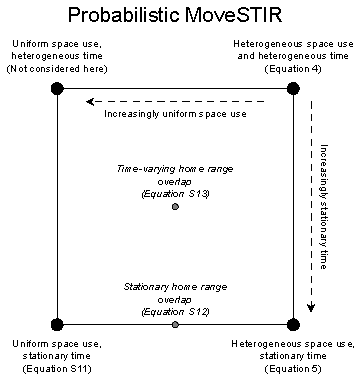
\includegraphics[width=\textwidth]{figures/conceptual_figure_pmovestir.pdf}
    \caption{Conceptual figure for PMoveSTIR}
\end{figure}

\end{document}
